\documentclass[tikz,border=5pt]{standalone}
\usepackage[utf8x]{inputenc}

\begin{document}

    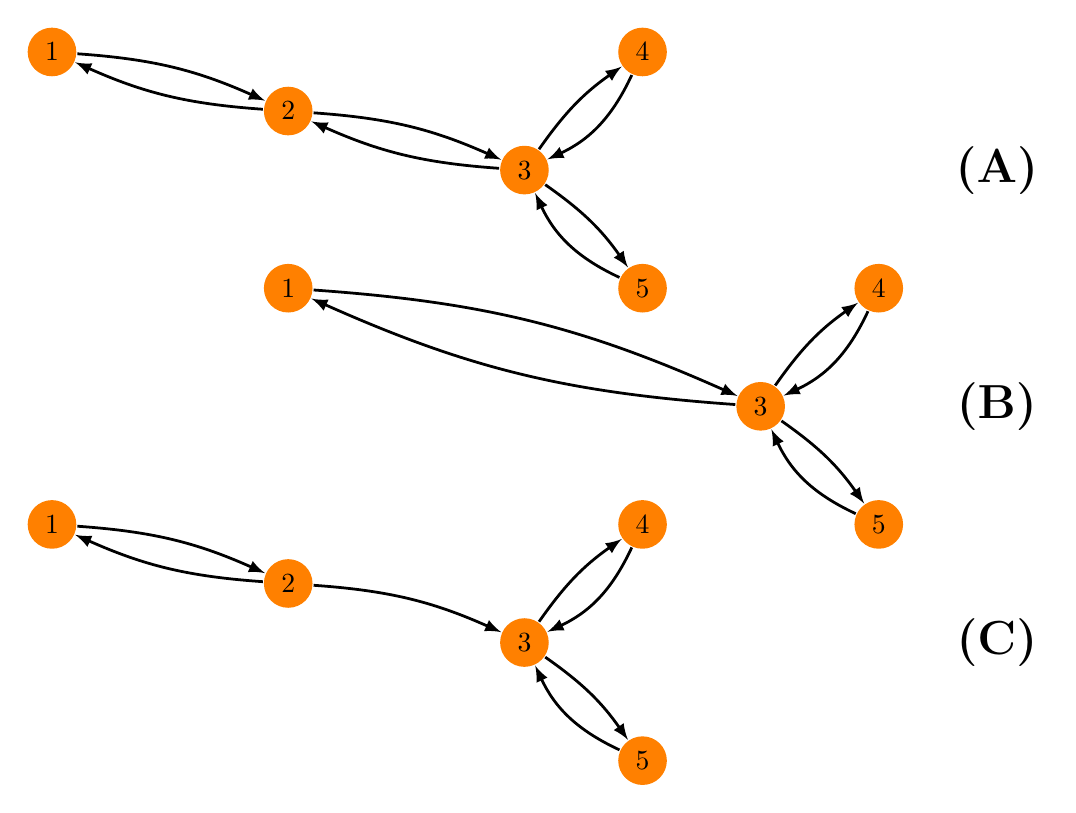
\begin{tikzpicture}[scale=3]
        \tikzstyle{node_style} = [thick, circle, fill=orange]
        \tikzstyle{arrow_style1} = [->, black, line width=1, >=latex]

        % This is (C) at the top
        \node[node_style] (n21) at (0,3) {1};
        \node[node_style] (n22) at (1,2.75) {2};
        \node[node_style] (n23) at (2,2.5) {3};
        \node[node_style] (n24) at (2.5,3) {4};
        \node[node_style] (n25) at (2.5,2) {5};

        \draw[arrow_style1] (n21) edge [bend left=10] (n22);
        \draw[arrow_style1] (n22) edge [bend left=10] (n21);
        \draw[arrow_style1] (n22) edge [bend left=10] (n23);
        \draw[arrow_style1] (n23) edge [bend left=10] (n22);
        \draw[arrow_style1] (n23) edge [bend left=10] (n24);
        \draw[arrow_style1] (n24) edge [bend left=20] (n23);
        \draw[arrow_style1] (n23) edge [bend left=10] (n25);
        \draw[arrow_style1] (n25) edge [bend left=20] (n23);

        % Then (B) in the middle
        \node[node_style] (n1) at (1,2) {1};
        %\node[node_style] (n2) at (2,1.75) {2};
        \node[node_style] (n3) at (3,1.5) {3};
        \node[node_style] (n4) at (3.5,2) {4};
        \node[node_style] (n5) at (3.5,1) {5};

        \draw[arrow_style1] (n1) edge [bend left=10] (n3);
        \draw[arrow_style1] (n3) edge [bend left=10] (n1);
        %\draw[arrow_style1] (n2) edge [bend left=10] (n3);
        %\draw[arrow_style1] (n3) edge [bend left=10] (n2);
        \draw[arrow_style1] (n3) edge [bend left=10] (n4);
        \draw[arrow_style1] (n4) edge [bend left=20] (n3);
        \draw[arrow_style1] (n3) edge [bend left=10] (n5);
        \draw[arrow_style1] (n5) edge [bend left=20] (n3);

        % Then (A) at the bottom
        \node[node_style] (n11) at (0,1) {1};
        \node[node_style] (n12) at (1,0.75) {2};
        \node[node_style] (n13) at (2,0.5) {3};
        \node[node_style] (n14) at (2.5,1) {4};
        \node[node_style] (n15) at (2.5,0) {5};

        \draw[arrow_style1] (n11) edge [bend left=10] (n12);
        \draw[arrow_style1] (n12) edge [bend left=10] (n11);
        \draw[arrow_style1] (n12) edge [bend left=10] (n13);
        %\draw[arrow_style1] (n13) edge [bend left=10] (n12);
        \draw[arrow_style1] (n13) edge [bend left=10] (n14);
        \draw[arrow_style1] (n14) edge [bend left=20] (n13);
        \draw[arrow_style1] (n13) edge [bend left=10] (n15);
        \draw[arrow_style1] (n15) edge [bend left=20] (n13);

        \node at (4, 2.5) {\bf\LARGE (A)};
        \node at (4, 1.5) {\bf\LARGE (B)};
        \node at (4, 0.5) {\bf\LARGE (C)};
    \end{tikzpicture}

\end{document}
